\appendix
\section{Technical Appendices and Supplementary Material}
\renewcommand\thefigure{S.\arabic{figure}}    
\setcounter{figure}{0}
\renewcommand\thetable{S.\arabic{table}}   
\setcounter{table}{0}

%%%%%%%%%%%%%%%% table of content %%%%%%%%%%%%%%%
\textbf{\Large Sections}

\begin{enumerate}
    \item Implementation Details for Self-Distillation (section~\ref{distillation})
    \item Implementation Details for Quantitative Evaluation (section~\ref{eval})
    \item Additional Efficiency Analysis of PH-Reg Compared to DVT (section~\ref{efficiency})
    \item Additional Qualitative Examples for Segmentation (section~\ref{additional})
    \item Additional Qualitative Heatmaps for PH-Reg Zero-Shot (section~\ref{denoising_supp})
    \item Proof of Test Time Augmentation  (section~\ref{proof})
\end{enumerate}
\newpage

\vspace{30em}

\section{Implementation Details for Self-Distillation}
\label{distillation}
% Please add the following required packages to your document preamble:
% \usepackage{graphicx}
\renewcommand{\arraystretch}{1.2}


In this section, we provide a detailed overview of how we implement self-distillation in PH-Reg. Our self-distillation framework consists of one teacher model and one student model. While both the teacher and student model are initialized from the same weights, the teacher is frozen, while additional register parameters are added to the student network. 

 Our codes and weights are avaible in \hyperlink{https://github.com/0raiser0/PH-Reg.git}{https://github.com/0raiser0/PH-Reg.git}. 


\subsection{Model Architectures}
\label{model}
\textbf{Teacher Model Architecture.}
For CLIP based models, since we focus on zero-shot open-vocabulary segmentation, we utilize the NACLIP modification to the final layer. This modification does not introduce any additional weights to the teacher network, and is training-free. Our empirical analysis in Section~\ref{pearson} shows that NACLIP's neighborhood attention mechanism improves feature consistency. For DINOv2, we directly use the final output layer, without any modification to the teacher network.


\textbf{Student Model Architecture.}
Based on the results from the ablation studies we integrate 16 register tokens into the student model. For the CLIP based student, to ensure representational alignment we directly take the \emph{v} head from the output layer (the MaskCLIP output). For DINO based students, we do not apply such modifications. We bicubicly upsample the positional embedding so it matches the input image. Unless otherwise specified, this modification is applied consistently, while all other layers remain unchanged.

%-----------------------
\subsection{Model Implementation}
\label{weights}

\begin{table*}[htbp]
\centering
\caption{\textbf{Model Implementation Libraries and Weights.} We compare models trained using different datasets and objectives.}
\vspace{.1cm}
\label{tab:weights}
\resizebox{\columnwidth}{!}{%
\begin{tabular}{l|l|l}
\hline
Model    & Library                   & Weight                                       \\ \hline
CLIP     & clip (OpenAI)             & ViT-B-16                                     \\
OpenCLIP & open\_clip                & hf-hub:laion/CLIP-ViT-B-16-laion2B-s34B-b88K \\
DFN-CLIP & open\_clip                & hf-hub:apple/DFN2B-CLIP-ViT-B-16             \\
DINOv2   & transformers (Hugging Face) & facebook/dinov2-base                         \\ \hline
\end{tabular}%
}
\end{table*}

We provide the model weights and the corresponding implementation libraries in Table~\ref{tab:weights}. 


\subsection{Optimization}
\label{opt}
In the distillation process, the shorter side of each input image is resized using bicubic interpolation to 448 for CLIP-based models and 518 for DINOv2. The resized image is then randomly cropped into a square of size (448, 448) or (518, 518), respectively. For each input image, we generate $N = 10$ augmentations using random shifts and horizontal flips. Assuming an image length of 1, we uniformly sample the shift for both the horizontal and vertical axes from $[-0.15, 0.15]$. While the horizontal flip is sampled with probability 0.5. To ensure each patch is covered, we do not apply any augmentation to the first image of the 10.  All shifted images are concatenated and fed into the teacher model, while the original (unshifted) images are used as input to the student model. The target feature is computed as the average of these 10 augmentations. To accommodate the resized input images for both the teacher and student models, we consistently resize the positional embeddings using bicubic interpolation. During training, the weights of the teacher model are frozen. In the student model, we allow updates to registers, the positional embeddings, the convolutional patch embedding layer, and the final transformer layer containing the self-attention mechanism.

The distillation framework is implemented in PyTorch, with distributed training managed via PyTorch Accelerate. Training is conducted on 4 NVIDIA Ada 6000 GPUs, with mixed-precision optimization to balance computational efficiency and numerical stability. Detailed training configurations are provided in Table~\ref{tab:clip_cfg} and Table~\ref{tab:dino_cfg}.

% Please add the following required packages to your document preamble:
% \usepackage{graphicx}
\renewcommand{\arraystretch}{1.2}
\begin{table*}[t]
\centering

\begin{minipage}[t]{0.48\textwidth}
\centering
\caption{Configs for CLIP-based models.}
\vspace{.1cm}
\resizebox{\linewidth}{!}{%
\begin{tabular}{l|l}
\hline
Config & Value \\ \hline
optimizer & AdamW \\
initial learning rate & 3e-4 \\
final learning rate & 1e-5 \\
weight decay & 1e-2 \\
optimizer momentum ($\beta_1, \beta_2$) & (0.9, 0.999) \\
learning rate scheduler & Exponential Scheduler \\
batch size & 16 \\
training epochs & 100 \\
augmentation & RandomSquareCrop \\ \hline
\end{tabular}%
}
\label{tab:clip_cfg}
\end{minipage}
\hfill
\begin{minipage}[t]{0.48\textwidth}
\centering
\caption{Configs for DINOv2.}
\vspace{.1cm}
\resizebox{\linewidth}{!}{%
\begin{tabular}{l|l}
\hline
Config & Value \\ \hline
optimizer & AdamW \\
initial learning rate & 1e-4 \\
final learning rate & 5e-6 \\
weight decay & 1e-2 \\
optimizer momentum ($\beta_1, \beta_2$) & (0.9, 0.999) \\
learning rate scheduler & Exponential Scheduler \\
batch size & 8 \\
training epochs & 100 \\
augmentation & RandomSquareCrop \\ \hline
\end{tabular}%
}
\label{tab:dino_cfg}
\end{minipage}

\end{table*}


\subsection{Pearson Analysis of Open-vocabulary Segmentation}\label{pearson}

\renewcommand{\arraystretch}{1.2}
\begin{table*}[h]
\centering
\caption{\textbf{Open-vocabulary Semantic Segmentation Quantitative Comparison on 7 datasets.} We report the Pearson correlation coefficient for the zero-shot query against the one-hot ground truth labels. The results are averaged within each image, then averaged across images. Compared to mIoU, pearson does not require knowledge of all of the categories present an image (via softmax). The value ranges from -1 to 1, where 1 = perfect positive correlation, -1 = perfect negative correlation, and 0 = no linear correlation. The best result for each dataset is highlighted in \textbf{bolded}.}
\vspace{.1cm}
\resizebox{\columnwidth}{!}{%
\begin{tabular}{l|ccccccccc}
\hline
Method        & VOC21          & PC60                    & VOC20          & PC59           & Stuff          & City           & ADE20k            & Avg.           \\ \hline
SCLIP         & -0.005         & 0.349                   & 0.409          & 0.443          & 0.323          & 0.291          & 0.308          & 0.303          \\
ClearCLIP     & 0.012          & 0.428                   & 0.489          & 0.543          & 0.393          & 0.336          & 0.418          & 0.374          \\
NACLIP      & 0.011          & 0.422                   & 0.470          & 0.543          & 0.392          & 0.363          & 0.425          & 0.375          \\
NACLIP+DVT    & 0.003          & 0.438                   & 0.487          & 0.551          & 0.395          & 0.367          & 0.427          & 0.381         \\
Ours (PH-Reg) & \textbf{0.013} & \textbf{0.468}          & \textbf{0.494} & \textbf{0.590} & \textbf{0.424} & \textbf{0.381} & \textbf{0.461} & \textbf{0.404} \\ \hline
\end{tabular}%
}
\vspace{-.2cm}
\label{tab:pearson}
\end{table*}
In this section we present additional evaluation results on open-vocabulary semantic segmentation via the pearson metric. Results are illustrated in Table~\ref{tab:pearson}. Overall, PH-Reg CLIP significantly outperforms the baseline models on 7 datasets. Even in the absence of prior category knowledge, PH-Reg CLIP achieves an average performance of 0.404, representing a clear improvement over the second-best method, DVT enhanced NACLIP, with an average performance of 0.381. 
These results highlight that our approach improves the consistency of dense feature representations by reducing artifact tokens, thereby offering a robust and generalizable enhancement over existing methods.

We further observe that both ClearCLIP and NACLIP achieve competitive results; however, NACLIP significantly outperforms ClearCLIP on ADE20K and Cityscapes. The former requires the model to handle a large number of categories, while the latter demands fine-grained localization of small objects. Based on this observation, we choose NACLIP as our primary teacher model, leveraging its neighbor attention mechanism to enhance the student model's performance on these challenging tasks.
\clearpage
\section{Implementation Details for Quantitative Evaluation}\label{eval}
In this section, we provide detailed implementation information for our quantitative evaluation experiments. 
In section~\ref{ovssimpl}, we present the evaluation details for open-vocabulary semantic segmentation (OVSS). In section~\ref{linearimpl}, we describe the evaluation details for linear probe based semantic segmentation and monocular depth estimation.

\subsection{Implementation Details of Open-vocabulary Semantic Segmentation.}
\label{ovssimpl}
We follow SCLIP and NACLIP in the setup for the open-vocabulary semantic segmentation evaluation. For fairness, we utilize the same parameters for all models. We resize input images such that the shorter side is scaled to a specific resolution, while maintaining the original aspect ratio for the longer side. Additionally, we set fixed crop sizes and strides during evaluation. All evaluation parameters are summarized in Table~\ref{tab:resize}, while all other settings follow their default configurations.

% Please add the following required packages to your document preamble:
% \usepackage{graphicx}
\renewcommand{\arraystretch}{1.2}
\begin{table*}[t]
\centering
\caption{\textbf{Dataset Specific Details for Open-vocabulary Semantic Segmentation.} We list the per-dataset resolution, crop size, and stride used for each dataset. We maintain the same settings for all methods within a given dataset.}
\vspace{.1cm}
\label{tab:resize}
\resizebox{\columnwidth}{!}{%
\begin{tabular}{l|cccccccc}
\hline
Dataset   & VOC21       & PC 60       & Object      & VOC20       & PC 59       & Stuff       & City        & ADE         \\ \hline
Resize resolution    & 448 & 448 & 336 & 336 & 448 & 448 & 560 & 448 \\
Crop size & 336         & 336         & 336         & 336         & 336         & 336         & 224         & 336         \\
Stride    & 112         & 112         & 112         & 112         & 112         & 112         & 112         & 112         \\ \hline
\end{tabular}%
}
\end{table*}

\subsection{Implementation Details of Linear Probe Based Evalution.}
\label{linearimpl}
Our linear probe evaluation follows prior works (Vision Transformers Need Registers, Denoising Vision Transformers), where a linear layer is trained as a decoding head to predict pixel-wise segmentation or depth logits.

\textbf{Semantic Segmentation.} We extract the final output features from the frozen backbone and, if applicable, pass them through the denoiser (for the DVT baseline). A single learnable linear layer is then trained to predict the segmentation logits. For CLIP-based models, both training and testing images are resized to (448, 448), while for DINOv2, the images are resized to (518, 518).

\textbf{Monocular Depth Estimation.}
Similar to semantic segmentation, we extract features from the backbone, and pass them through the denoiser if applicable. Following the method in DVT and DINOv2, we then append the \textbf{[CLS]} token to each patch token to enrich the feature representations for all methods. 
A linear layer is trained using SigLoss and gradient loss (scaled by a factor of 0.5) to predict depth values into 256 uniformly distributed bins. We adopt DVT's learning rate of 5e-3 for all experiments. 

\section{Additional Efficiency Analysis of PH-Reg Compared to DVT}\label{efficiency}
In this section, we provide a detailed efficiency analysis of PH-Reg compared to DVT, focusing on three aspects: training time, space usage, and inference cost.

% Please add the following required packages to your document preamble:
% \usepackage{graphicx}
\renewcommand{\arraystretch}{1.2}
\begin{table*}[t]
\centering
\caption{\textbf{Training Time Efficiency Analysis.} We report the training time of our PH-Reg method compared to DVT. For fairness, we restrict all stages of our model to a single GPU and evaluate the same model (DINOv2 ViT-B).}
\vspace{.1cm}
\resizebox{\columnwidth}{!}{%
\begin{tabular}{l|cccc}
\hline
Method & Stage 1 Extraction & Stage 1 Distillation & Stage 2 Training & Total               \\ \hline
DVT    & 2998 min           & 18340 min            & 570 min          & 21908 min (365.1 h) \\
PH-Reg & -                  & -                    & -                & 9000 min (150 h)    \\ \hline
\end{tabular}%
}
\label{tab:training}
\vspace{-.2cm}
\end{table*}
\textbf{Training Time.} When evaluating training time, we utilize the official code provided in the DVT repository without any modification. The original DVT code specifies a single GPU for feature extraction and learning – for fairness we also limit all stages of our own model to a single GPU here. For DVT and PH-Reg, we evaluate the same model (DINOv2 ViT-B).
Results are illustrated in Table~\ref{tab:training}. Our method has the advantage of not utilizing gradient-based neural field learning as done in DVT. Therefore, our method trains the student model in a single stage, saving over 58.9\% of the time compared to DVT.


\textbf{Space Usage.} A further advantage is the space utilization during training. DVT requires saving 1.4 terabytes of intermediate neural fields in the form of serialized Instant-NGP files. Our method computes all distillation targets on the fly, and requires no additional space.

% Please add the following required packages to your document preamble:
% \usepackage{graphicx}
\renewcommand{\arraystretch}{1.2}
\begin{table*}[t]
\centering
\caption{\textbf{Inference Efficiency Analysis.} We report the inference cost results for all models, evaluating efficiency based on model size and GFLOPs.}
\vspace{.1cm}
\resizebox{0.6\columnwidth}{!}{
\begin{tabular}{l|cc}
\hline
Method                                 & GFLOPs & Params (M) \\ \hline
MaskCLIP                               & 62.89  & 86.19      \\
NACLIP                                 & 64.76  & 86.19      \\
NACLIP w/ denoising (10x) & 647.6  & 86.19      \\
NACLIP + DVT                             & 70.32  & 94.07      \\
CLIP + PH-Reg (Ours)                   & 64.16  & 86.66 \\
\hline
\end{tabular}
}
\label{tab:inference}
\vspace{-.2cm}
\end{table*}
\textbf{Inference Cost.} When evaluating testing cost for all models, we cast parameters to \emph{fp32} dtype, and use eager attention implementation for all models. For our method, we include the positional embeddings adapted for 448 resolution. For MaskCLIP and NACLIP, current official implementations have the same number of parameters as the original CLIP, although a small reduction can be achieve in MaskCLIP by discarding the last \emph{q, k} head.
For DVT, we evaluate their stage 2 model, corresponding to the transformer block denoiser coupled to a original vision transformer.
Results are illustrated in Table~\ref{tab:inference}. Our method utilizes approximately 10\% fewer FLOPs and 10\% fewer parameters during inference compared to DVT. 




\clearpage

\section{Additional Qualitative Examples}
\label{additional}

\begin{figure}[htbp]
  \centering
  \vspace{-1em}
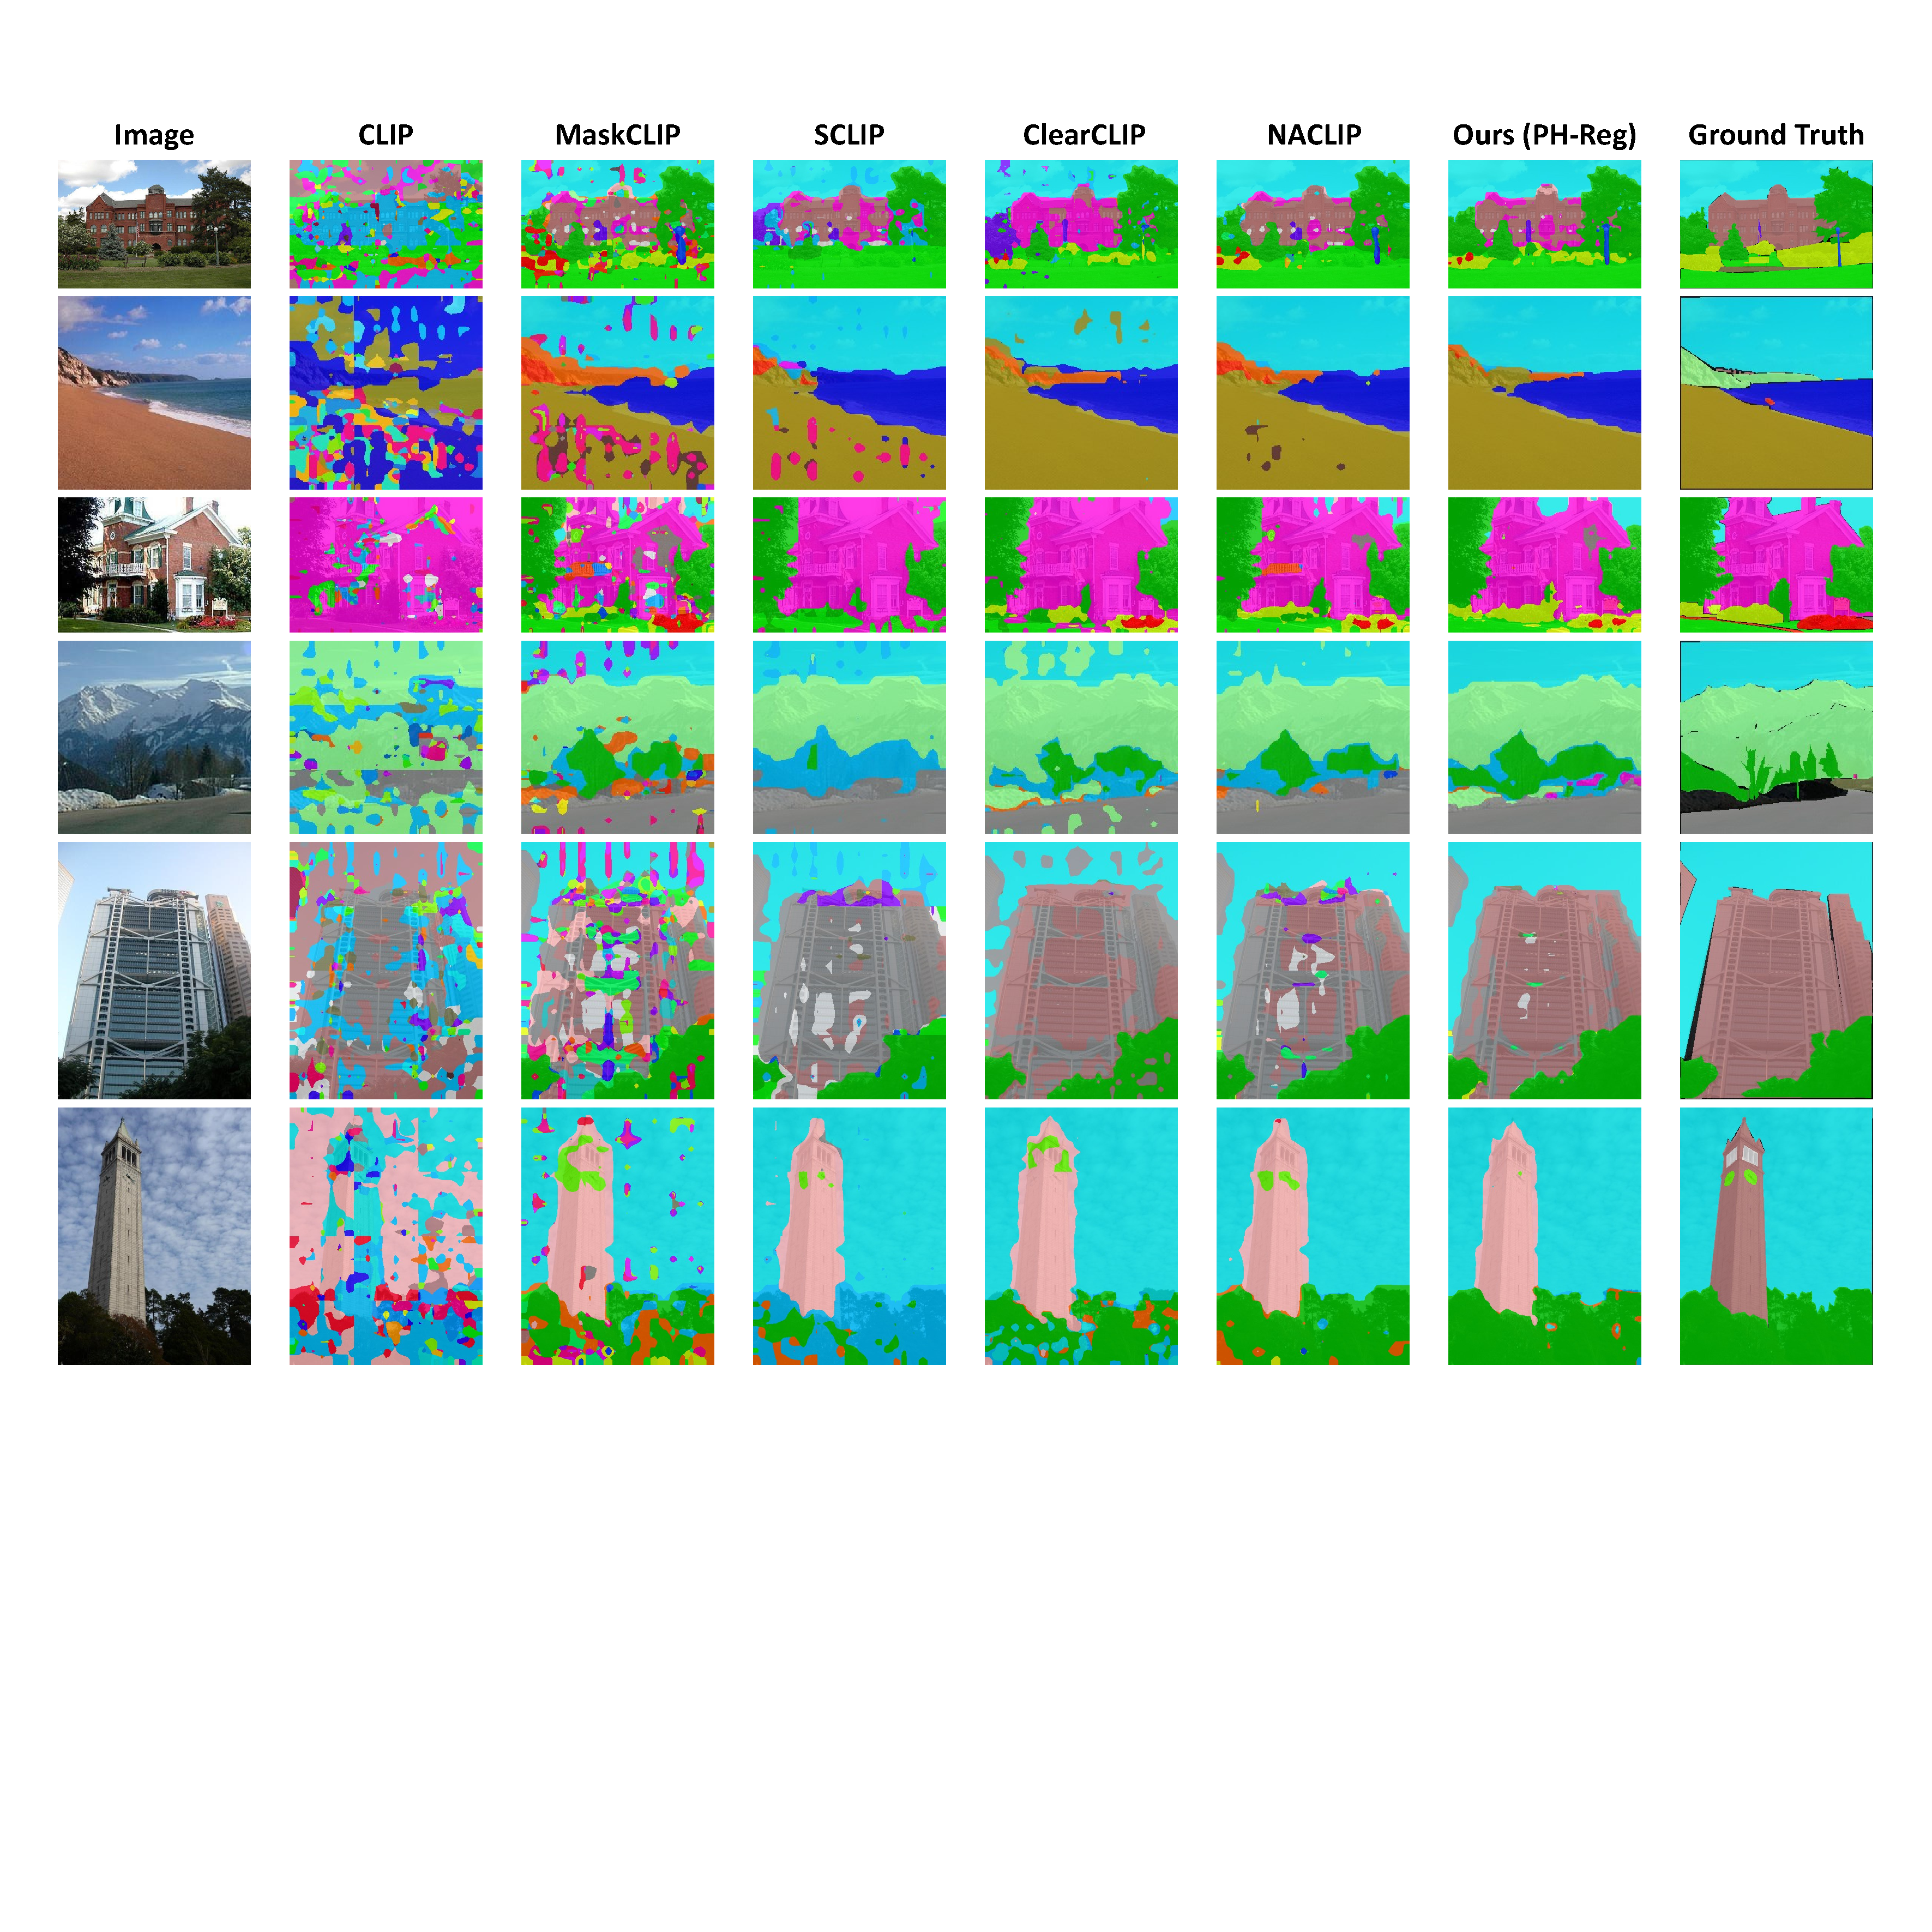
\includegraphics[width=0.95\linewidth, trim=0 470 0 0, clip]{fig_pdf/ade20k.pdf}
  \caption{Open-vocabulary semantic segmantation qualitative comparision between different baseline models on ADE20K.}
  \vspace{-.5cm}
  \label{fig:ade}
\end{figure}

\begin{figure}[htbp]
\vfill
  \centering
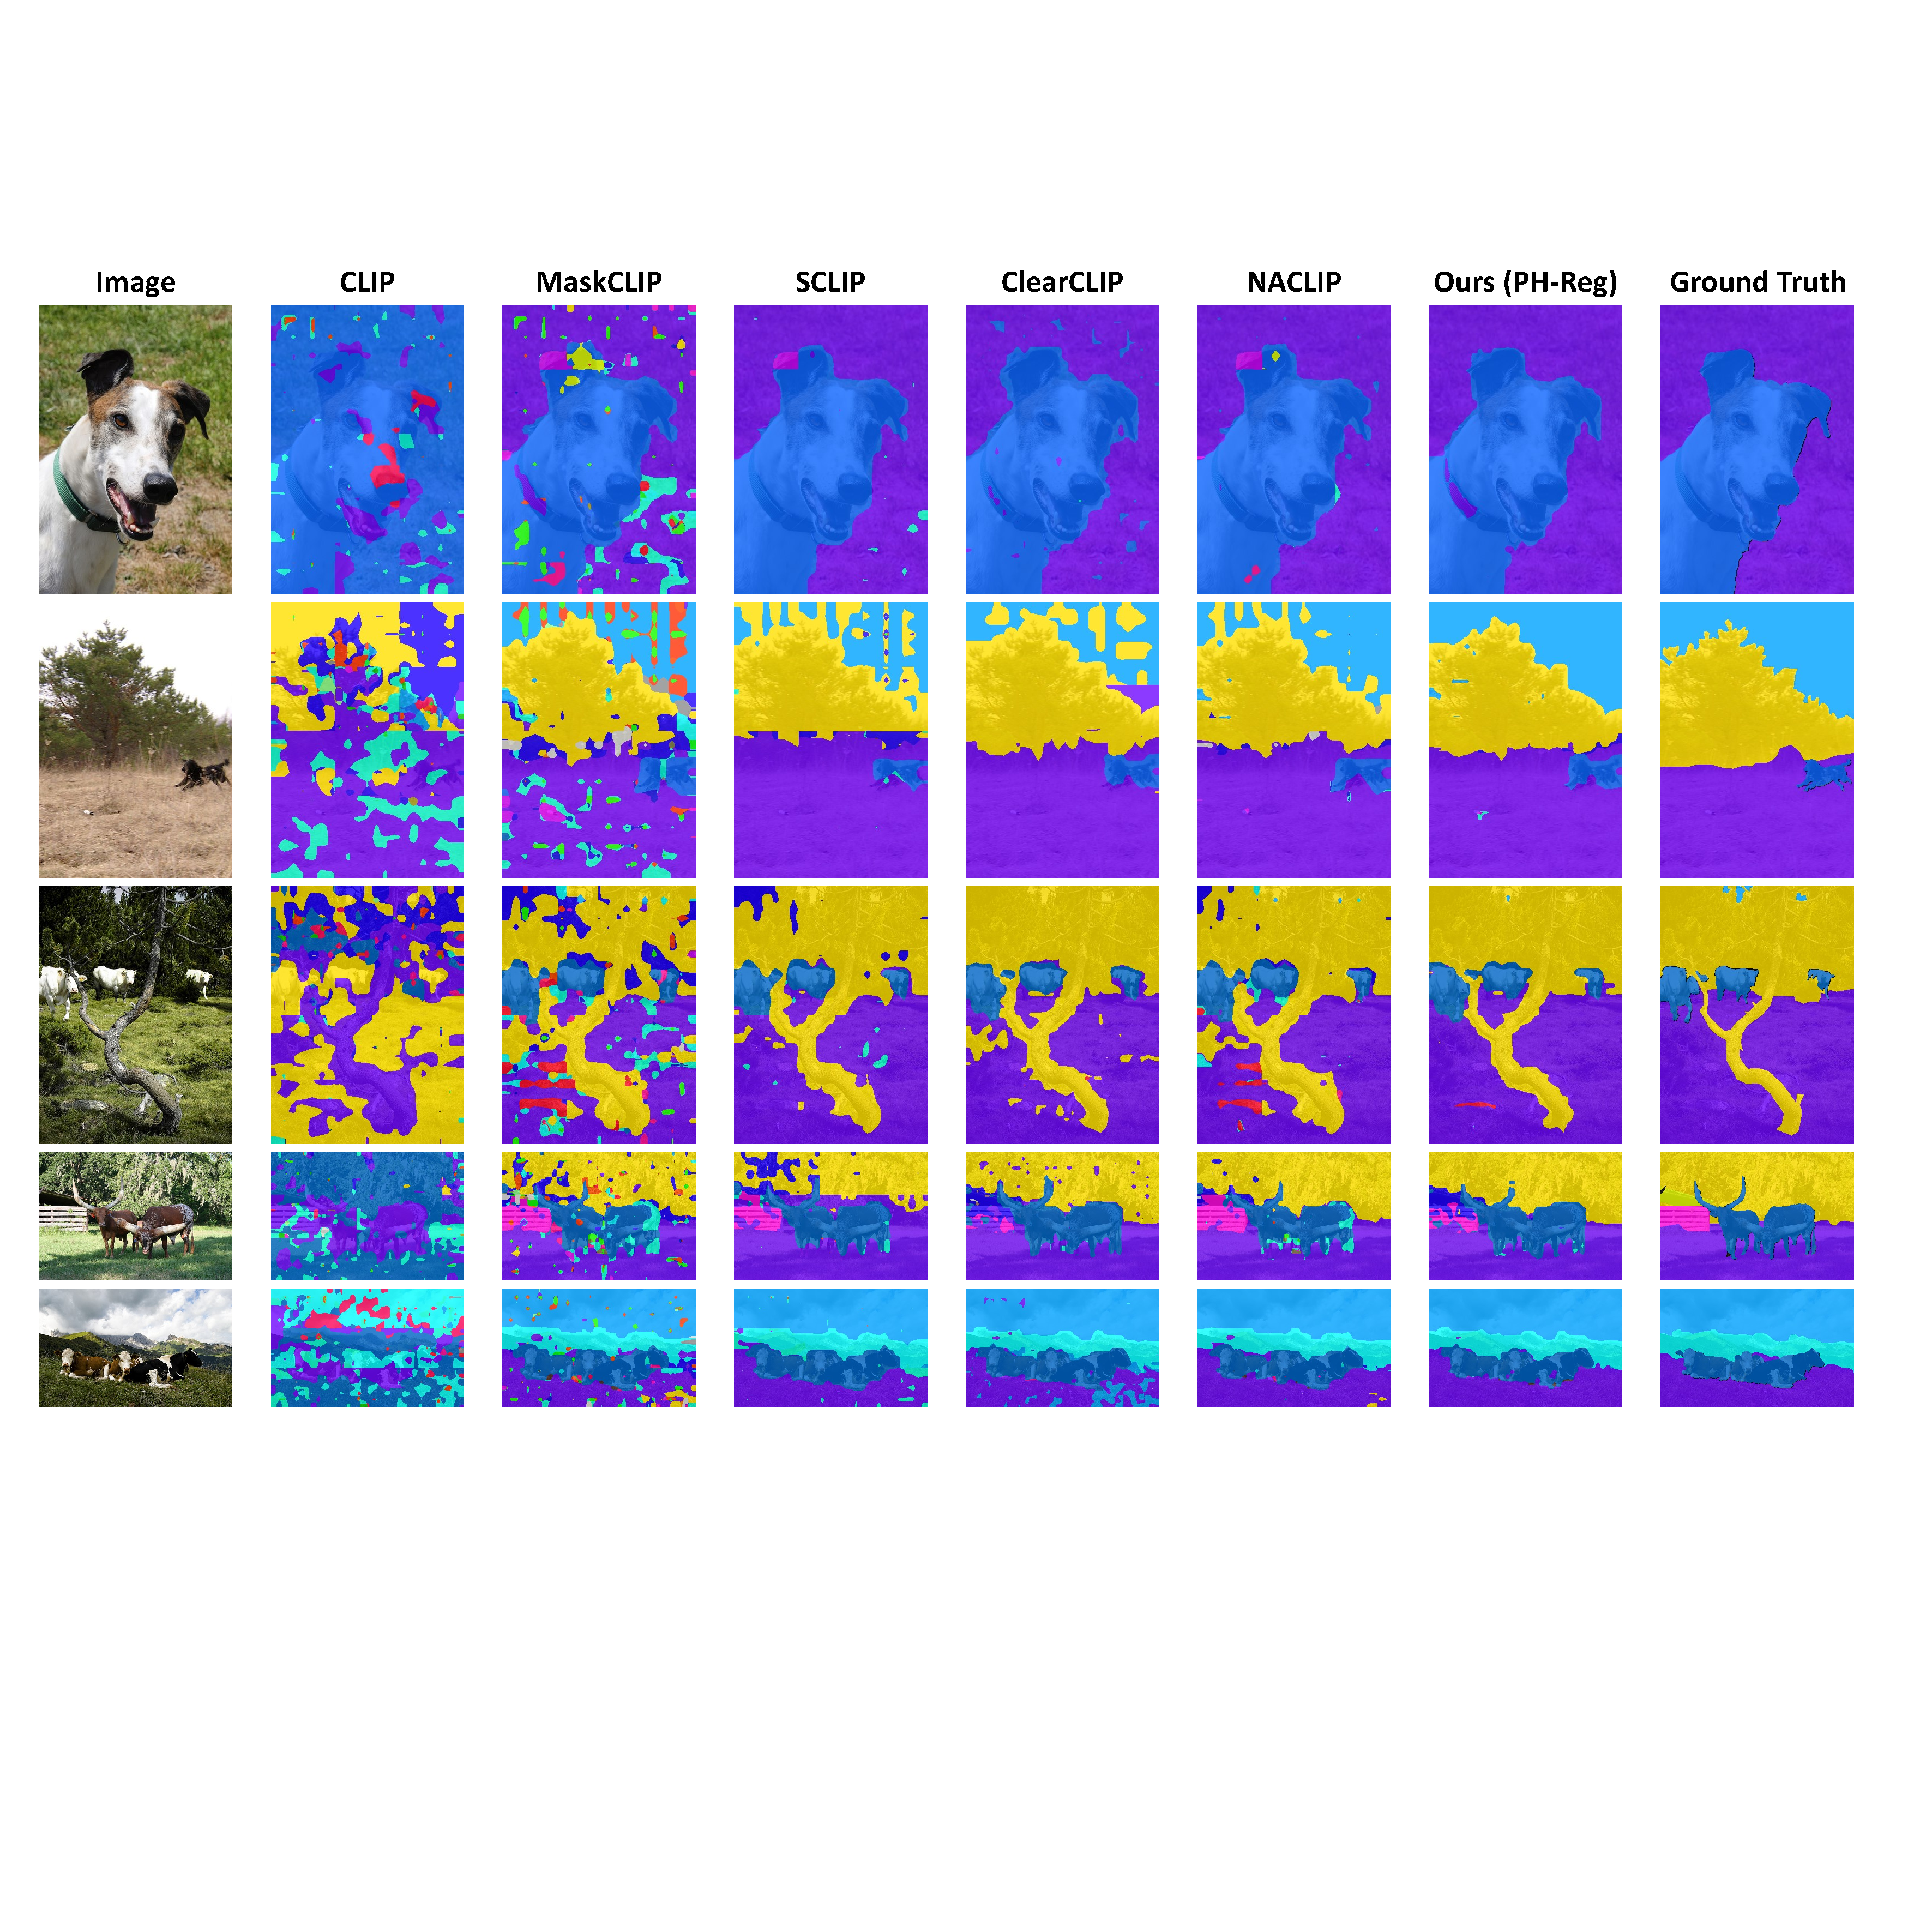
\includegraphics[width=0.95\linewidth, trim=0 450 0 140, clip]{fig_pdf/context59.pdf}
  \caption{Open-vocabulary semantic segmantation qualitative comparision between different baseline models on Pascal Context59.}
  \vspace{-.5cm}
  \label{fig:voc}
\vfill
\end{figure}
\newpage

\begin{figure}[htbp]
  \centering
  % \vspace{-2em}
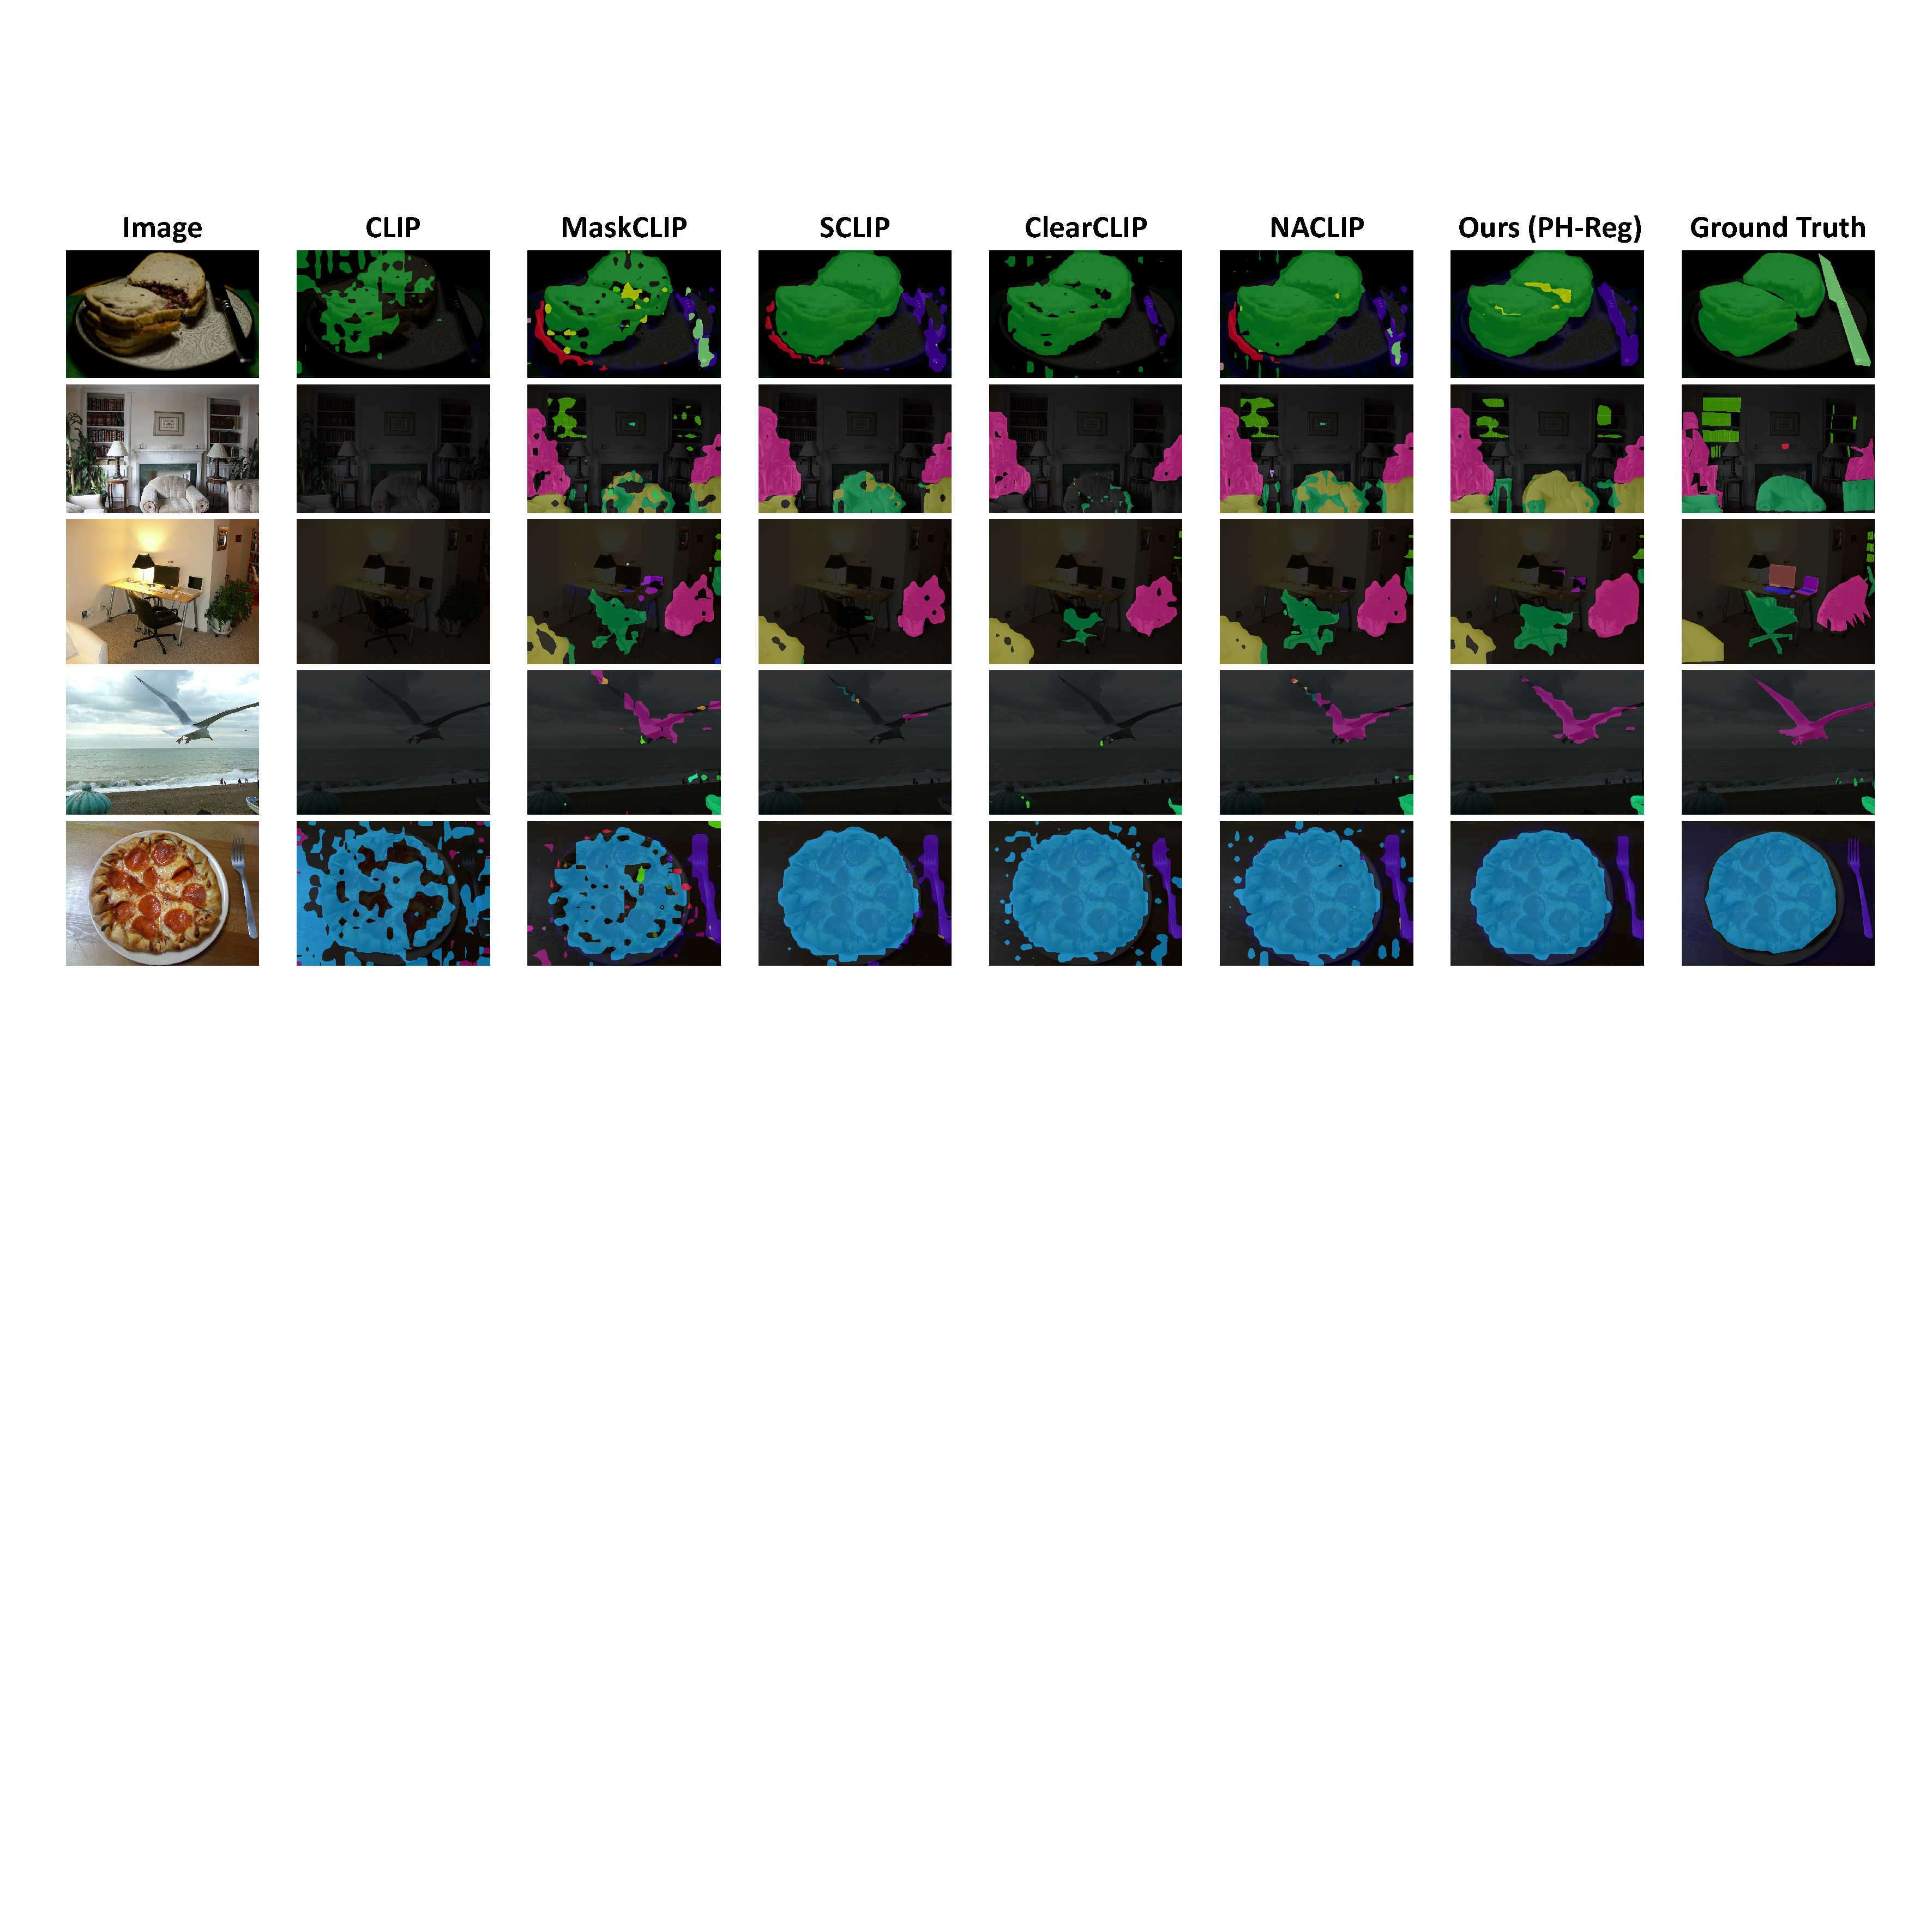
\includegraphics[width=0.95\linewidth, trim=0 850 0 100, clip]{fig_pdf/object.pdf}
  \caption{Open-vocabulary semantic segmantation qualitative comparision between different baseline models on COCO Obejct.}
  \vspace{-.5cm}
  \label{fig:obj}
\end{figure}

\clearpage

\section{Additional Qualitative Heatmaps for PH-Reg Zero-Shot}\label{denoising_supp}
\begin{figure}[htbp]
\vfill
  \centering
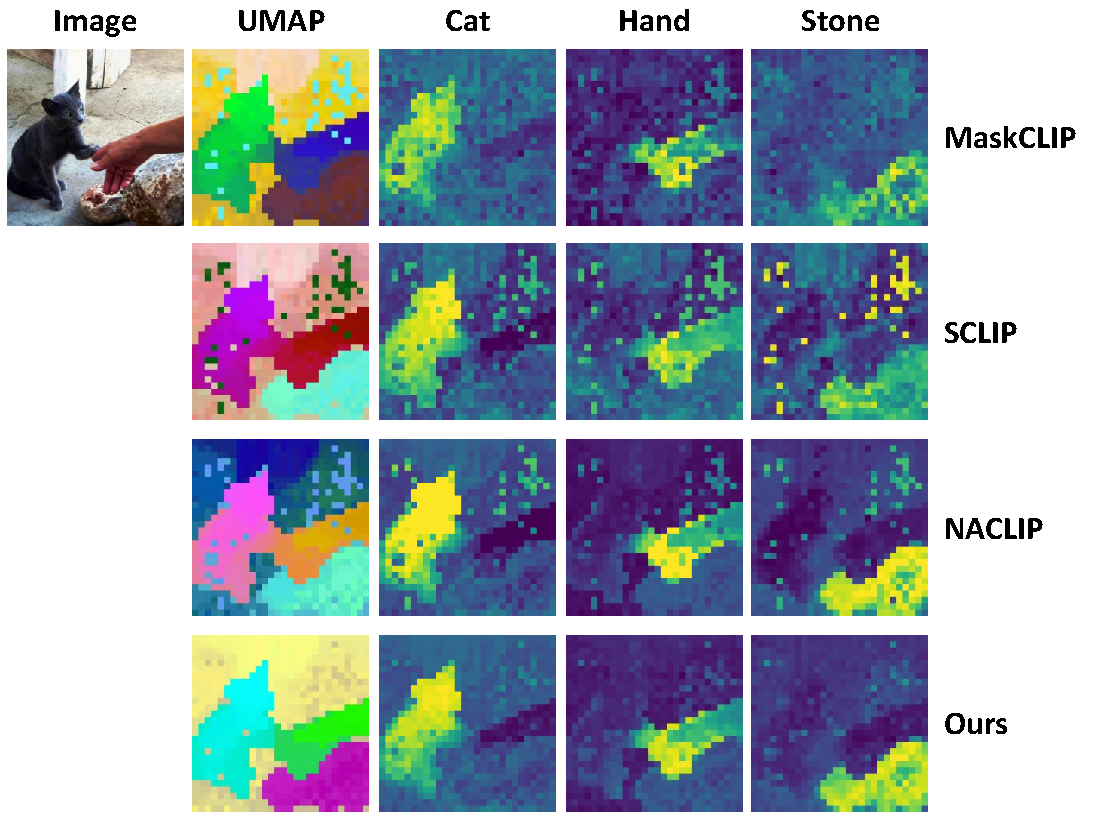
\includegraphics[width=0.85\linewidth]{fig_pdf/sim1_1.pdf}
  \caption{\textbf{Zero-shot Heatmap Results.} Our results have fewer artifacts than other methods.}
  \vspace{-.5cm}
\vfill
\end{figure}

\begin{figure}[htbp]
\vfill
  \centering
  \vspace{1cm}
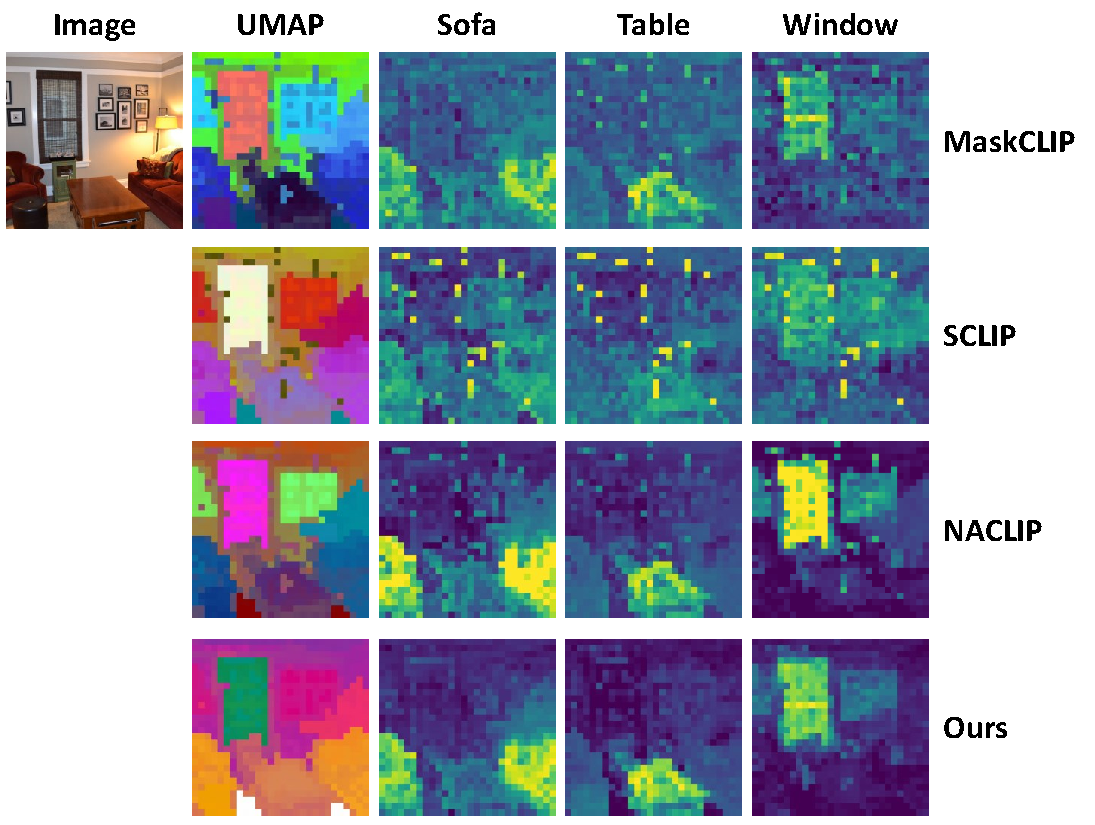
\includegraphics[width=0.85\linewidth]{fig_pdf/sim1_2.pdf}
  \caption{\textbf{Zero-shot Heatmap Results.} Our results have fewer artifacts than other methods.}
  \vspace{-.5cm}
\vfill
\end{figure}
\clearpage

\begin{figure}[htbp]
\vfill
  \centering
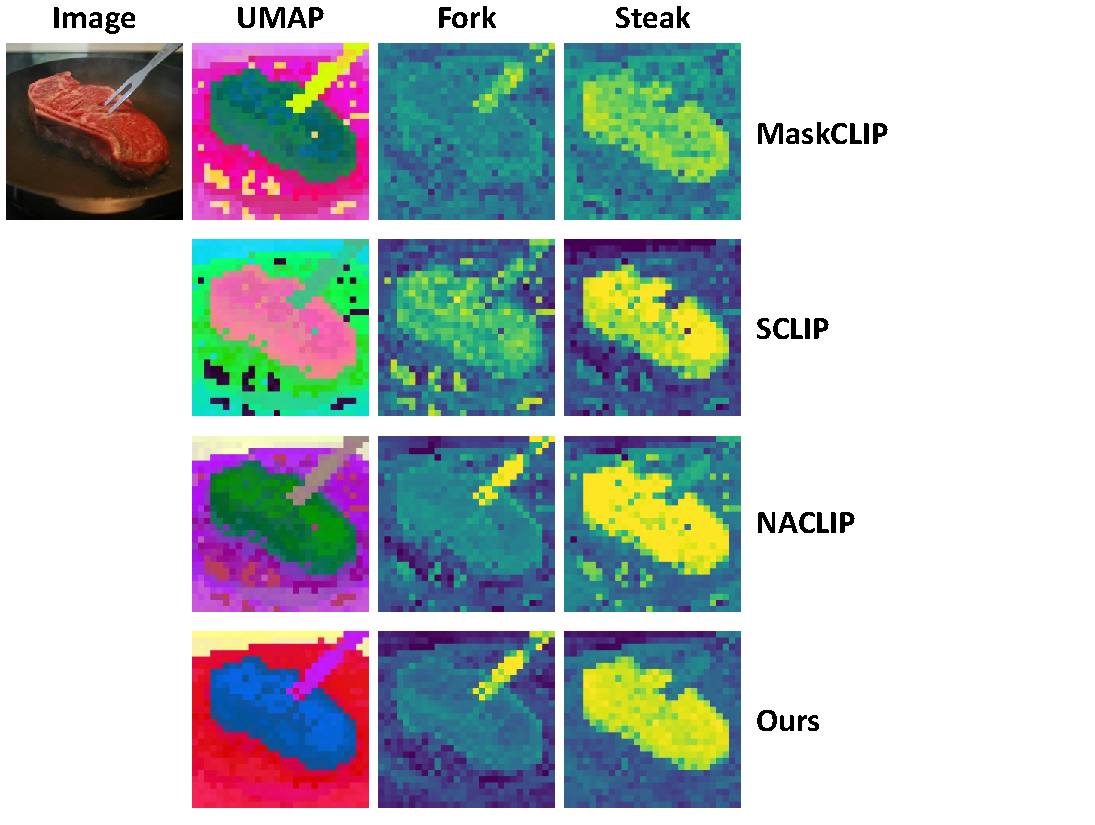
\includegraphics[width=0.85\linewidth]{fig_pdf/sim2_1.pdf}
  \caption{\textbf{Zero-shot Heatmap Results.} Our results have fewer artifacts than other methods.}
  \vspace{-.5cm}
\vfill
\end{figure}

\begin{figure}[htbp]
\vfill
  \centering
  \vspace{1cm}
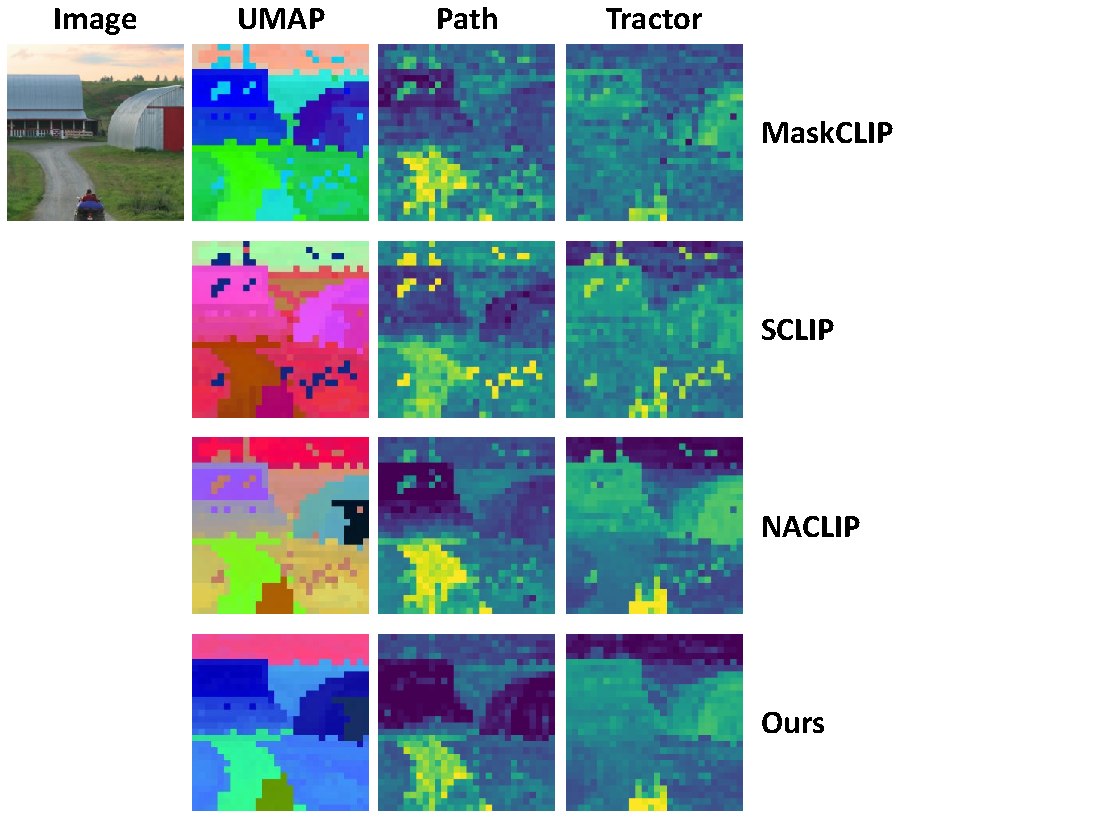
\includegraphics[width=0.85\linewidth]{fig_pdf/sim2_2.pdf}
  \caption{\textbf{Zero-shot Heatmap Results.} Our results have fewer artifacts than other methods.}
  \vspace{-.5cm}
\vfill
\end{figure}

\clearpage


\section{Optimal Feature Aggregation}
\label{proof}
Let $ f_{1}, \dots, f_{n} \in \mathbb{R}^d$ be feature vectors of a single patch from $n$ different transformations of an input image $\mathcal{I}$. We seek the optimal aggregated feature $f^*$ that minimizes the total squared error:

\begin{equation}
f^* = \mathop{\arg\min}_{f} \sum_{i=1}^n \|f_i - f\|_2^2
\end{equation}

Expanding the objective gives us:
\begin{equation}
\mathop{\arg\min}_f\sum_{i=1}^n (f_i^\top f_i - 2f_i^\top f + f^\top f)
\end{equation}

Dropping constant terms that do not change the optimum:
\begin{equation}
= nf^\top f - 2\left(\sum_{i=1}^n f_i^\top\right) f
\end{equation}
Dividing and multiplying the right side by $n$:
\begin{equation}
= nf^\top f - 2n\left(\sum_{i=1}^n \frac{1}{n} f_i^\top\right) f
\end{equation}
Dividing the equation by $n$ as whole shows us that we need to minimize:
\begin{equation}
\|f-\frac{1}{n}\sum_{i=1}^{n} f_i\|_{2}^{2}
\end{equation}
So it can be derived that the mean of the feature vectors is the minimizer under MSE loss: 

\begin{equation}f^* = \frac{1}{n}\sum_{i=1}^{n} f_i\end{equation}



